\chapter{Blockchain}
\section{Blokchain 1.0}
La blockchain è un database completamente decentralizzato, in cui ogni nodo possiede una replica e concorda, sulla base di un algoritmo comune, un’unica versione aggiornata delle informazioni. Si tratta di una struttura dati nella quale è possibile solo aggiungere nuovi dati, senza possibilità di cancellare quelli precedenti, garantendo così uno storico completo delle modifiche.
\\Per chiarire meglio questo concetto, possiamo immaginare la blockchain come una barriera corallina: lo strato attivo corrisponde alla parte più recente, che viene continuamente modificata con nuove aggiunte, mentre gli strati più vecchi rimangono immutabili e accessibili solo per attività di consultazione.
Può essere quindi rappresentata come una lista in continua crescita di “blocchi”, collegati tra loro e protetti mediante crittografia. 
\\Oltre alla decentralizzazione e all’immutabilità, il terzo grande punto di forza è il consenso: nuove transazioni possono essere registrate solo quando la maggioranza dei partecipanti alla rete dà il proprio consenso.
\\I blocchi sopra citati sono composti da 7 campi principali: 
\vspace{1em}
\begin{adjustwidth}{1cm}{0pt}
    \begin{itemize}[itemsep=1ex]
        \item[\textbullet\ \textit{Block} $\rightarrow$ ]  rappresenta il numero del blocco all'interno della blockchain. Ogni volta che un nuovo blocco viene aggiunto, questo numero aumenta progressivamente;
        \item[\textbullet\ \textit{Nonce} $\rightarrow$ ]  è un valore, spesso composto da 32 bit (come nel caso di Bitcoin), fondamentale perché viene cercato dai miner per generare un hash valido che soddisfi i requisiti di difficoltà della chain. Serve a modificare l’input del calcolo dell’hash e viene aggiornato continuamente durante il processo di mining;
        \item [\textbullet\ \textit{Timestamp} $\rightarrow$ ] indica il momento esatto in cui il blocco è stato aggiunto alla blockchain;
        \item [\textbullet\ \textit{Transaction} $\rightarrow$ ] contiene o un valore (ad esempio un importo monetario), o il corpo del messaggio, o uno smart contract;
        \item [\textbullet\ \textit{Transaction n} $\rightarrow$ ] si riferisce a una specifica transazione tra le diverse transazioni presenti all’interno del blocco;
        \item [\textbullet\ \textit{Prev Hash} $\rightarrow$ ] è l’hash del blocco precedente, che funge da chiave di collegamento tra i blocchi. Questo meccanismo garantisce che ogni blocco sia dipendente dal precedente, creando una catena ininterrotta;
        \item [\textbullet\ \textit{Hash} $\rightarrow$ ] rappresenta l’impronta digitale del blocco. È un valore alfanumerico unico calcolato applicando una funzione hash. L’hash è deterministico, nel senso che lo stesso input produrrà sempre lo stesso hash; tuttavia, non è possibile risalire ai dati originali partendo dall’hash. Ogni minima modifica ai dati genera un hash completamente diverso, garantendo così l’integrità e l’immutabilità delle informazioni.
    \end{itemize}
\end{adjustwidth}
\vspace{1em}
\begin{figure}[t]
    \centering
    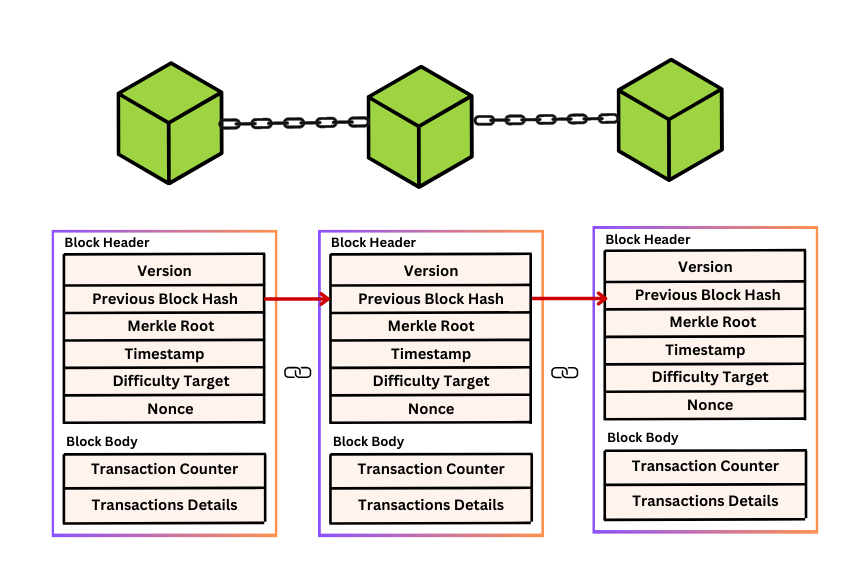
\includegraphics[width=0.8\textwidth]{Immagini/structure of block.png}
    \caption{Esempio di catena}
\end{figure}
\subsection{Bitcoin}

L’aspetto rivoluzionario di Bitcoin è la creazione di una forma monetaria completamente decentralizzata. La sua rete è composta da una serie di componenti chiamate nodi, che collaborano tra loro per raggiungere il consenso su una sequenza di transazioni.
Essendo basato sulla blockchain, Bitcoin è completamente decentralizzato: non è gestito da un’entità centrale, come avviene per esempio con le banche. 
\\Questo comporta un vantaggio significativo, ovvero una maggiore resistenza a comportamenti anomali o malintenzionati. In un sistema centralizzato, infatti, il nodo centrale rappresenta un punto di vulnerabilità che potrebbe compromettere l’intero sistema.
\\Un’altra caratteristica fondamentale di Bitcoin è la disintermediazione: ogni transazione coinvolge direttamente il mittente e il destinatario che raggiungono il consenso tramite l’approvazione della rete. Bitcoin è quindi costituito da una rete di sistemi indipendenti, i nodi, capaci di mantenere un registro univoco e condiviso delle transazioni. Questo sistema garantisce che un singolo bitcoin non possa essere speso più di una volta.\\
In tal modo, Bitcoin soddisfa le funzioni critiche di ogni valuta:
\begin{itemize}
\item immagazzinare valore;
\item essere un’entità contabile;
\item trasferire valore tra le parti.
\end{itemize}
La sua blockchain è di tipo permissionless, il che significa che chiunque può eseguire il software del nodo e collegarsi alla rete senza alcuna forma di autenticazione. In altre parole, chiunque può unirsi alla rete senza necessità di approvazioni o permessi da parte di un’autorità centrale.
\\Un elemento fondamentale è il wallet che consente agli utenti di gestire i propri bitcoin, conservati in veri e propri conti. Ogni bitcoin è associato a un address, protetto da una coppia di chiavi crittografiche.
La chiave pubblica rappresenta l’indirizzo del conto ed è accessibile a tutti, mentre la chiave privata rappresenta l’identità del proprietario ed è necessaria per accedere e autorizzare le transazioni.
\\Bitcoin utilizza la crittografia asimmetrica, un sistema inventato nel 1976 da Whitfield Diffie e Martin Hellman. Questo metodo permette di cifrare con una chiave (pubblica) un messaggio che può essere decifrato solo con l’altra chiave (privata), e viceversa, ciò determina due vantaggi principali.
Il primo è l'Hashing e il secondo è la firma digitale.
\\L'hashing trasforma qualsiasi quantità di dati in una stringa cifrata di dimensioni fisse, chiamata digest e comporta numerosi vantaggi in quanto è: 
\vspace{1em}
\begin{adjustwidth}{1cm}{0pt}
    \begin{itemize}[itemsep=1.5ex]
        \item[\textbullet\ \textit{deterministico} $\rightarrow$ ] lo stesso input produce sempre lo stesso digest;
        \item [\textbullet\ \textit{a lunghezza fissa} $\rightarrow$ ] il digest ha una lunghezza predeterminata, indipendentemente dalla dimensione dell’input;
        \item [\textbullet\ \textit{unico} $\rightarrow$ ] è estremamente improbabile che due input diversi generino lo stesso digest;
        \item [\textbullet\ \textit{non invertibile} $\rightarrow$ ] è impossibile risalire all’input originale partendo dal digest;
        \item [\textbullet\ \textit{instabile} $\rightarrow$ ] una minima modifica all’input genera un digest completamente diverso.
    \end{itemize}
\end{adjustwidth}
\vspace{1em}
L'altro grosso vantaggio è la firma digitale che garantisce unicità e non ripudiabilità. 
\\Quando un utente X invia a un utente Y un messaggio firmato digitalmente, X crea l’hash del messaggio e lo cifra con la propria chiave privata. Y, ricevendo il messaggio, può verificare l’hash con la chiave pubblica di X, garantendo così l’integrità del messaggio e la validità del mittente.
\begin{figure}[h]
\centering
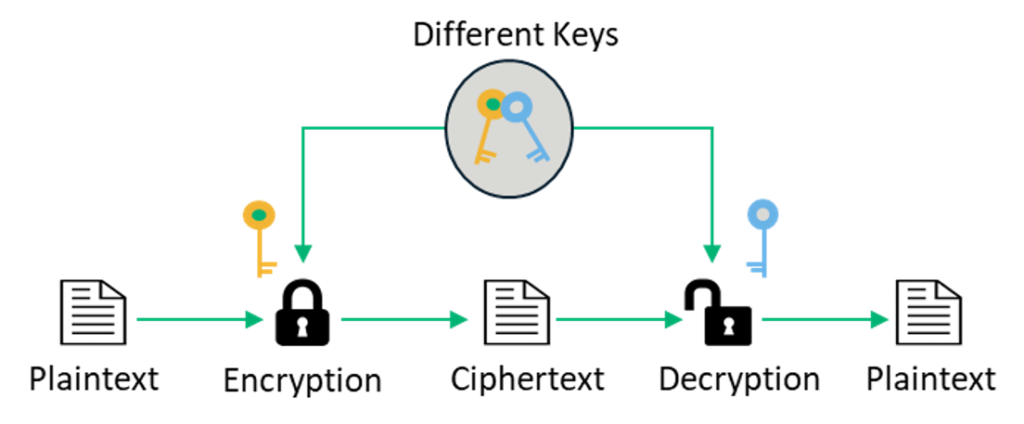
\includegraphics[width=0.65\textwidth]{Immagini/cifratura asimmetrica.png}
\caption{Esempio di cifratura asimettrica}
\end{figure}
\\
Bitcoin è open source, il suo codice sorgente è pubblico e rilasciato sotto licenza MIT, che permette la massima libertà di utilizzo per progetti futuri.
\\Nonostante il grande successo riscosso, Bitcoin presenta diverse criticità che ne limitano l'efficacia e l'adozione su larga scala. Una delle principali problematiche riguarda la scalabilità: l'algoritmo Proof of Work (PoW) su cui si basa il sistema, pur garantendo sicurezza, tende a limitare l'efficienza complessiva, rendendo difficile gestire un alto numero di transazioni in tempi brevi.
Un altro aspetto delicato è quello relativo a privacy e visibilità. Sebbene gli account su Bitcoin siano pseudonimi, tutte le transazioni effettuate sulla rete sono pubblicamente visibili. Questo permette, tramite un'analisi approfondita dei movimenti della valuta, di risalire potenzialmente all'identità dei possessori, mettendo in discussione la reale riservatezza del sistema.
La difficoltà di aggiornamento rappresenta un'ulteriore sfida. Il complesso sistema di governance che coinvolge minatori, sviluppatori e utenti, rende particolarmente arduo raggiungere un consenso per apportare modifiche al protocollo. Ciò può rallentare l'implementazione di miglioramenti necessari.
\\Infine vi è il problema delle commissioni elevate, che si verifica nei periodi di intenso utilizzo della rete. In queste circostanze, effettuare transazioni rapide può diventare molto costoso, specialmente se il tasso di cambio tra Bitcoin ed Euro è particolarmente alto.

\newpage
\subsection{Proof Of Work}
Come accennato in precedenza, la sicurezza e la validità delle transazioni in Bitcoin sono garantite da un algoritmo di consenso chiamato Proof of Work (PoW) \cite{Blockchain_guida_allecosistema}. Un algoritmo di consenso è un protocollo condiviso da tutti i nodi della rete che consente loro di concordare su una visione unica delle transazioni.
\\In primo luogo, ogni nodo condivide con gli altri nodi della rete le transazioni ricevute nell’ultimo intervallo di tempo, firmate digitalmente. Successivamente ciascun nodo costruisce in memoria un elenco delle transazioni ricevute dagli altri nodi con cui è in comunicazione. Queste transazioni vengono ordinate e viene verificato che ogni account disponga dei fondi necessari per completare i pagamenti.
A questo punto, i nodi partecipano a una competizione crittografica per individuare, in modo casuale, il nodo che avrà il diritto di pubblicare il blocco successivo. Quando un nodo vince la competizione, individua un blocco valido e lo comunica a tutti gli altri nodi. Questi ultimi verificano il blocco e lo aggiungono alla propria copia della blockchain.
\begin{figure}[h]
\centering
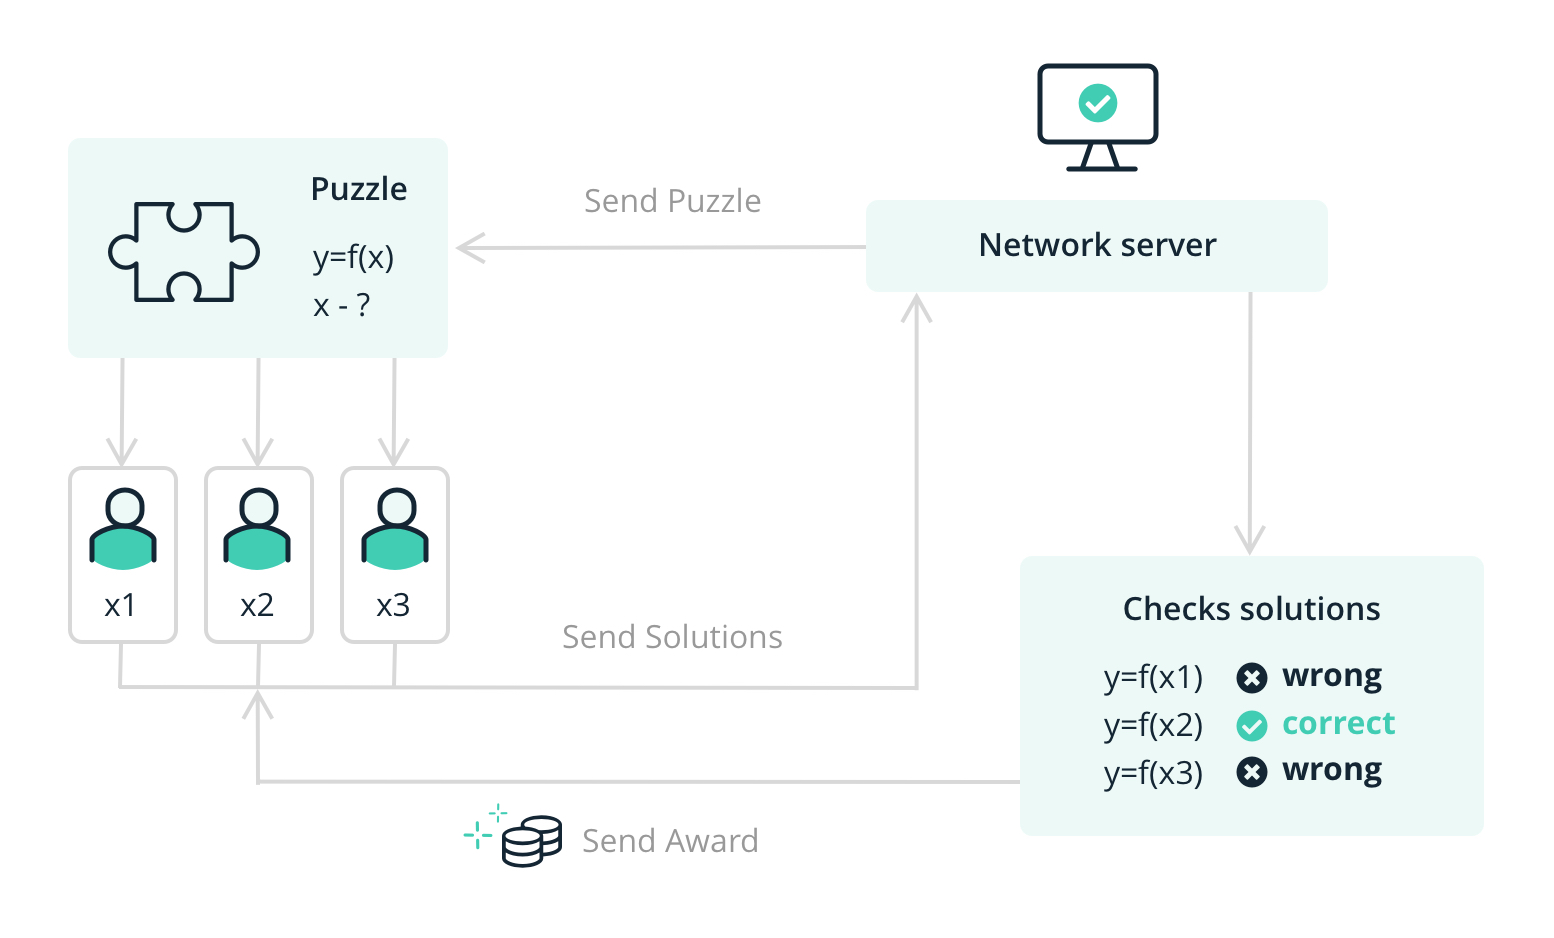
\includegraphics[width=0.65\textwidth]{Immagini/proof of work scheme.jpg}
\caption{Esempio di funzionamento del PoW}
\end{figure}
\\
In questo ambito si sente spesso parlare di fork \cite{Blockchain_tecnologia_e_applicazioni_per_il_business}, ma non è sempre chiaro cosa si intenda con questo termine e cosa effettivamente comporti. Sebbene venga spesso utilizzato per indicare la divisione di una blockchain, in realtà esso racchiude un insieme di diversi possibili scenari. 
\\Una fork è una situazione in cui si verifica uno dei seguenti scenari:
\begin{itemize}
    \item può accadere che due o più nodi trovino contemporaneamente una soluzione valida. In tal caso si generano due blocchi con lo stesso genitore, creando una biforcazione nella catena, detta fork. Quando viene individuato il blocco successivo, l’algoritmo seleziona la catena più lunga (in termini di difficoltà complessiva) come valida. Questo caso viene denominato come fork regolare;
    \item le regole della Blockchain sono cambiate in maniera retrocompatibile e tutti i nodi condividono la stessa cronologia delle transazioni, in questo caso si tratta di soft fork e non c’è una divisione della blockchain;
    \item le regole della Blockchain sono cambiate in maniera non retrocompatibile, ma tutti i nodi si aggiornano alle nuove regole e condividono la stessa cronologia delle transazioni, anche in questo caso non si ha una divisione della blockchain, ma si tratta di un hard fork;
    \item le regole della blockchain sono cambiate in maniera non retrocompatibile e nodi diversi hanno opinioni diverse sulle regole della blolckchain, non condividendo la stessa cronologia delle transazioni, abbiamo quindi un hard fork con chain split, dato che avviene una divisione della chain e il consenso sulla cronologia delle transazioni e perso definitivamente.
\end{itemize}
Questo criterio, basato sul "principio di maggior lavoro", permette a tutti i nodi di concordare su una versione univoca della blockchain e di risolvere le biforcazioni. Un blocco viene considerato finalizzato, quando sono stati generati almeno sei blocchi successivi. Questo livello di profondità rende economicamente insostenibile, per una minoranza di nodi malintenzionati, modificare i dati della blockchain, poiché richiederebbe un effort computazionale estremamente elevato pari al 51\% della potenza totale di calcolo del network e, anche se ipoteticamente un miner riuscisse a raggiungere tale potenza, non sarebbe comunque in grado di modificare le vecchie transazioni, poiché dovrebbe ricalcolare la PoW di tutti i blocchi successivi, mentre gli altri miner onesti continuano a minare sulla blockchain corretta. Un attacco di questo tipo richiederebbe l’utilizzo di una quantità incredibile di risorse per l’attacker. Se qualcuno effettivamente riuscisse a mettere insieme più del 51\% della potenza di calcolo, sarebbe molto più redditizio per lui seguire le regole della blockchain.
Nonostante i numerosi vantaggi che il Proof of Work offre, questo algoritmo di consenso presenta alcune significative criticità. La principale è il massiccio consumo di energia, un aspetto che, paradossalmente, costituisce anche uno dei suoi punti di forza, rendendo estremamente costoso e complesso attaccare la rete.
A questo si aggiunge la scarsa scalabilità del sistema che si traduce in una certa lentezza nell’elaborazione delle transazioni e nell’aumento delle commissioni, soprattutto nei periodi di maggiore attività sulla rete. Infine il Proof of Work tende a creare una sorta di discriminazione geografica: attualmente, la maggior parte dei miner si concentra in aree dove il costo dell’elettricità è più basso, limitando la partecipazione globale e accentuando disparità economiche e infrastrutturali \cite{Blockchain_tecnologia_e_applicazioni_per_il_business}.

\section{Blokchain 2.0}

\subsection{Ethereum e Proof Of Stake}
Bitcoin, per sua natura, non è stato concepito come un ambiente di sviluppo e offre funzionalità di programmazione molto limitate, mentre la community ha sempre voluto mantenere la piattaforma focalizzata sullo scambio di valori, lasciando spazio a progetti alternativi che miravano ad ampliare le possibilità della tecnologia blockchain.
\\È in questo scenario che nasce Ethereum, la prima blockchain progettata specificamente per supportare lo sviluppo di applicazioni decentralizzate. Co-fondata nel 2013 da Vitalik Buterin, un programmatore russo-canadese che in passato aveva collaborato con Bitcoin Magazine, Ethereum si distingue da Bitcoin per molteplici innovazioni.
\\Una delle principali novità introdotte è la possibilità di utilizzare due tipi di conti: quelli tradizionali posseduti tramite una coppia di chiavi pubblica e privata, come in Bitcoin e quelli associati agli Smart Contract \cite{Blockchain_guida_allecosistema}. 

\subsection{Smart Contracts}
Gli Smart Contract, concettualizzati per la prima volta da Nick Szabo nel 1994, sono programmi in grado di eseguire automaticamente azioni predeterminate una volta soddisfatte certe condizioni.
\begin{figure}[h]
    \centering
    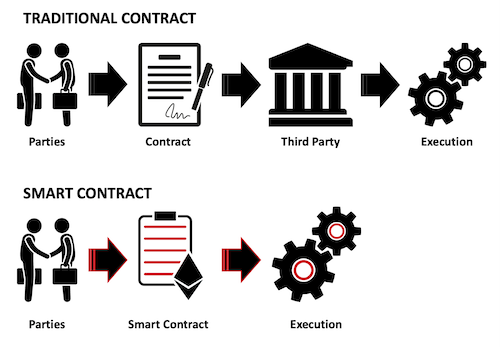
\includegraphics[width=0.65\textwidth]{Immagini/smart-contract.png}
    \caption{Esempio di Smart Contract}
\end{figure}
Questi contratti decentralizzati garantiscono che le regole siano rispettate senza la necessità di intermediari, eliminando possibili interferenze.
\\Un esempio pratico di utilizzo degli Smart Contract è il crowdfunding. Un utente potrebbe pubblicare un progetto stabilendo un obiettivo economico e un tempo limite per raggiungerlo. Lo Smart Contract, in questo caso, si occuperebbe di raccogliere i fondi dagli investitori e trattenerli fino al completamento della campagna. Se l’obiettivo viene raggiunto, i fondi vengono trasferiti automaticamente al creatore del progetto; in caso contrario, tornano ai donatori. 
\\Questa struttura elimina la necessità di intermediari e rende il processo completamente trasparente.
Ethereum utilizza Solidity, un linguaggio di programmazione simile a JavaScript, per scrivere Smart Contract; la flessibilità offerta da questa piattaforma ha rivoluzionato il mondo delle blockchain, permettendo la creazione di applicazioni decentralizzate e inaugurando l’era delle cosiddette blockchain 2.0.

\subsection{Vantaggi e svantaggi del PoS}
Inizialmente veniva utilizzato il meccanismo di consenso Proof of Work (PoW), lo stesso di Bitcoin, però per migliorare efficienza e sostenibilità, il 15 settembre 2022, con l’aggiornamento noto come The Merge, Ethereum è passato al Proof of Stake (PoS). 
Questo cambiamento ha segnato un cambio epocale per la piattaforma ed ha portato con se enormi vantaggi \cite{crypto_gateway_video}.
\\Il PoS riduce drasticamente il consumo energetico, abbassandolo del 99,9\% rispetto al PoW, ed elimina la necessità di hardware costoso per il mining, rendendo la partecipazione al consenso più accessibile.
Con l’introduzione del PoS, Ethereum ha reso possibile lo staking, un processo in cui i partecipanti bloccano una quantità di criptovaluta in uno Smart Contract per sostenere la sicurezza e il funzionamento della blockchain. Attraverso lo staking, gli utenti possono diventare validatori e partecipare attivamente alla convalida delle transazioni e alla creazione di nuovi blocchi.
\\Lo staking offre numerosi vantaggi: aumenta la sicurezza del sistema rendendo gli attacchi costosi e difficili da eseguire, favorisce la decentralizzazione permettendo a più utenti di contribuire alla rete e riduce il consumo energetico rispetto al mining tradizionale. 
I partecipanti allo staking ricevono ricompense proporzionali alla loro attività sotto forma di nuove criptovalute o ottengono una parte delle commissioni generate dalle transazioni.
Le ricompense non si limitano ai validatori che propongono nuovi blocchi, ma includono anche coloro che verificano e confermano la validità dei blocchi proposti da altri. Questo sistema rende lo staking una delle principali motivazioni per partecipare al consenso su Ethereum, favorendo un equilibrio tra efficienza e incentivi economici.
Inoltre, il sistema garantisce una maggiore scalabilità e permette ai validatori onesti di proteggere la rete da attacchi, penalizzando economicamente i nodi malevoli o inattivi per almeno il 50\% del tempo attraverso un meccanismo chiamato slashing che risulterà totale per i primi andando a sottrarre in maniera permanente le risorse depositate nello stake, mentre sarà parziale per i secondi che si vedranno sottratti solo i guadagni ricevuti ma non saranno rimossi dalla chain.
\\Nonostante questi vantaggi, il PoS presenta alcune criticità. Essendo una tecnologia più recente rispetto al PoW è meno testata e potrebbe essere più vulnerabile a eventi imprevisti, i cosiddetti Black Swan. Inoltre, il fatto che il controllo della rete sia legato al possesso di criptovalute pone un rischio di centralizzazione: chi dispone di maggiori capitali potrebbe accumulare una quantità significativa di token, aumentando la propria influenza sul sistema \cite{kraken_docsend}.
